\section{Agile \& Kanban}

Agil betyder forandringsparathed.
Centrale værdier for agil softwareudvikling.

Individer og interaktioner er vigigere end processer og værktøjer. Software, der virker, er vigtigere end omfattende dokumentation.
Samarbejde med kunden er vigtigere end kontraktforhandling. At kunne reagere på forandringer er vigtigere end at følge en plan.


\textbf{The agile enterprise}
\begin{itemize}
	\item{Der skal være en stærk virksomhedsideologi}
	\item{Der skal være en stærk virksomhedskultur med afsæt i ideologien.}
	\item{Man skal kunne agere proaktivt.}
	\item{Man skal kunne reagere reaktivt.The agile enterprise}
	\item{Forandringsparathed skal kunne måles}
	\item{Virksomheden skal råde over en række genbrugelige komponenter, som nemt kan kombineres.}
	\item{Ovennævnte plug-in kompatibilitet understøttes aktivt af udviklende standarder.}
	\item{Medarbejderne skal kunne eksperimentere frit i selvorganiserende grupper}
	\item{Virksomheden skal facilitere videndeling.}
	\item {Koordinering finder sted på individniveau}
\end{itemize}

\textbf{Kanban}
Kanban er en metode til at styre flowet af arbejdet. Man bruger "noter" på "tavler" til at visualisere og holde styr på projektet.

\begin{center}
	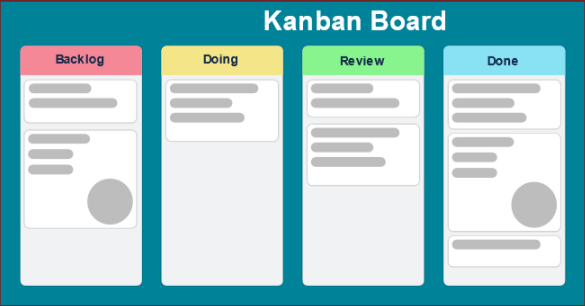
\includegraphics[width=0.8\textwidth]{Images/Kanban.png}
\end{center}

Ved Kanban har man et commitment point, hvor vi beslutter os for at det skal udføres.
Dertil er der lead time, som er hvor lang tid det tager at gennemføre. En vigtig begrænsing er  WIP limits.
Work in progress limits sikrer at man færdiggører opgaver og ikke bare tilføjer flere.

